\chapter{Design}
\label{sec:design}

% Ist das zentrale Kapitel der Arbeit. Hier werden das Ziel sowie die
% eigenen Ideen, Wertungen, Entwurfsentscheidungen vorgebracht. Es kann
% sich lohnen, verschiedene Möglichkeiten durchzuspielen und dann
% explizit zu begründen, warum man sich für eine bestimmte entschieden
% hat. Dieses Kapitel sollte - zumindest in Stichworten - schon bei den
% ersten Festlegungen eines Entwurfs skizziert werden.
% Es wird sich aber in einer normal verlaufenden
% Arbeit dauernd etwas daran ändern. Das Kapitel darf nicht zu
% detailliert werden, sonst langweilt sich der Leser. Es ist sehr
% wichtig, das richtige Abstraktionsniveau zu finden. Beim Verfassen
% sollte man auf die Wiederverwendbarkeit des Textes achten.

% Plant man eine Veröffentlichung aus der Arbeit zu machen, können von
% diesem Kapitel Teile genommen werden. Das Kapitel wird in der Regel
% wohl mindestens 8 Seiten haben, mehr als 20 können ein Hinweis darauf
% sein, daß das Abstraktionsniveau verfehlt wurde.

%%%%%%%%%%%%%%%%%%%%%%%%%%%%%%%%%%%%%%%%%%%%%%%%%%%%%%%%%%%%%%%%%%%%%%%%%%%%%%%%
%                                                                              %
% MOTIVATION AND REQUIREMENTS                                                  %
%                                                                              %
%%%%%%%%%%%%%%%%%%%%%%%%%%%%%%%%%%%%%%%%%%%%%%%%%%%%%%%%%%%%%%%%%%%%%%%%%%%%%%%%
\section{Motivation}
\begin{itemize}
% Overall motivation of a communication layer
\item Parallel computers are stricly necessary in scientific community
\item Parallel computers are compute clusters
  \ref{sec:cluster} with a very homogeneous layout, in which the nodes
  are connected by a abitrary network.  Usually application domain is
  decomposed \ref{sec:domain_decomposition} in smaller chunks
  of work and then distributed onto the homogenous network of nodes on
  the cluster.  So to speak a very heterogeneous phyisical simulation
  is mapped onto a homogeneous compute architecture.

  This is fine as long the simulation is not changing to much during
  runtime. Thus every node stays utilized. But instead real world
  simulations are changing over time. The workload could increase
  globally or only locally on some subdomains of the simulation
  volume.

  This leads to an unbalanced load during the simulation and therefore
  to unutilized ressource of the compute cluster. In this cases it
  could make sense to start some new domain decomposition or it could
  also make sense to move whole subdomains from one node to another.

  This all needs a powerful communication layer which is flexibel
  enough to support such rebalancing of workload. Common cluster
  communication frameworks are not able to fullfill these
  requirements. They are usually static in their distribution and do
  not satisfy our needs.

  \todo{State out that communication layer should be exchangeable}

\item PIConGPU \ref{sec:picongpu} is even harder because of an
  hierarchicle memory architecture.
\item NUMA architecture will crow even harder
\end{itemize}

% Requirements
\subsection{Requirements}
To be able to model such complex and heterogeneous topologies the
following components are required:

\begin{itemize}
\item Communication abstraction layer, which introduce an abstraction
  from existig communication layers.
\item Description of the communication topology
\item Possibility to communicate inside the physical domain
\item Mapping of communiation topology onto the hardware topology
\end{itemize}

%%%%%%%%%%%%%%%%%%%%%%%%%%%%%%%%%%%%%%%%%%%%%%%%%%%%%%%%%%%%%%%%%%%%%%%%%%%%%%%%
%                                                                              %
% ANALYSIS OF PIConGPU CODE                                                    %
%                                                                              %
%%%%%%%%%%%%%%%%%%%%%%%%%%%%%%%%%%%%%%%%%%%%%%%%%%%%%%%%%%%%%%%%%%%%%%%%%%%%%%%%
\section{Analysis of PIConGPU-Code}
\begin{itemize}
  \item How does the communication topologie looks like ?
  \item What are the different levels of communication ?
  \item What kind of communcation layer is used ?
  \item How is Communication implemented in PIConGPU ?
\end{itemize}

%%%%%%%%%%%%%%%%%%%%%%%%%%%%%%%%%%%%%%%%%%%%%%%%%%%%%%%%%%%%%%%%%%%%%%%%%%%%%%%%
%                                                                              %
% COMMUNICATION ABSTRACTION LAYER                                              %
%                                                                              %
%%%%%%%%%%%%%%%%%%%%%%%%%%%%%%%%%%%%%%%%%%%%%%%%%%%%%%%%%%%%%%%%%%%%%%%%%%%%%%%%
\section{Abstraction from Existing Communication Layers}
\todo{mention policy based design}
\todo{Wie trägt komponente bei motivation zu erfüllen}

% Motivation for communication abstraction
Applications can be interconnected by vast variety of communication
libraries. But it can not be assumed that every cluster system
supports every communication library on the market.  Thus, the
abstraction from existing communication libraries is a fundamental
property for a flexibel and portable application.

Even though, that there are existing standards for communication in
cluster systems, the world of computer science is subject to constant
change. Thus the possibility to exchange the used communication layer
without changing the interface to this layer, is a precondition for
future applications in distributed computing.

The challange is to provide a very general interface, that is able to
map varying communication libraries onto it. This interface should not
be modeled from the scratch, instead it should remind the interface
user on known communication methods. It should be deployable into existing
applications by replacing the actual communication library without
changing the understanding of the fundamental way to communicate in
this application.

This section presents the design of a generic communication layer
which fulfils the before discussed requirements.

% Brief CAL description
\subsection{Communication Abstraction Layer (CAL)}
The \textit{Communication Abstraction Layer}, shortly \textit{CAL}, is
a generic interface that provides access to a varity of communication
libraries. The libraries are available as adapters, which can be
configured at compile time (Figure \ref{fig:cal}).

\begin{figure}[H]
  \centering \includegraphics[width=0.8\textwidth]{graphics/30_cal}
  \caption{Communication Abstraction Layer (CAL)}
  \label{fig:cal}
\end{figure}

Using the CAL instead of a concrete communication library has the
advantage that in the case of a changing communication environment
(e.g migrating to another cluster) only the adapter has to be
exchanged and the application has to be recompiled, but the CAL does
not change.

\subsection{Addressing of Peers}
% CAL virtual addressing
Communication libraries come with their own address schema, which can
be quiete different. Socket based systems address their peers by ip
addresses, where MPI based systems address their processes by ranks.
These diverse ways to address peers in a network need to be translated
to an unified address space. Each CAL provides a virtual address
which is an unique identifier for its peer in the adapters network.

The address space of the virtual address are natural numbers in 
the range from 0 to the number of peers minus one. This addressing
schema is the simplest way and satifies the needs of the actual design.

% CAL interface
\subsection{Communication Interface}

% Peer2Peer Operations
\subsubsection{Peer to Peer Operations}
In the first place the CAL provides peer-to-peer communication. That
are basic communication operations to send and receive abitrary data
between two peers. These operations are available both blocking and
non-blocking. The interface is influenced by existing communication
libraries that all share a common interface ( e.g.boost::mpi,
boost::asio, ZMQ). The core interface for sending and receiving data:

\begin{itemize}
  \item send(destination, tag, data)
  \item recv(source, tag, data)
\end{itemize}

\begin{description}
\item[Data] \hfill \\
  The data that should be transmitted to
  another peer or that should be received from another peer.  The data
  object should provide a function data() that returns the pointer to a
  contigiuous memory area and a function size() that returns the size
  of the object. The STL sequence containers std::vector and
  std::array allready support these functions at least since C++ version
  C++11.
\item[Destination / Source] \hfill \\
  This is the virtual address of the sending or receiving peer.
\item[Message Tag] \hfill \\
  The message tag is an unsigned interger that gives
  a message a meaning similar to headers of communication
  protocols. Thus, it helps a peer to distinguish between messages of
  the same sending peer.
\end{description}

It is not planed in the actual design that the CAL provides routing
abilities. Peers have to be connected directly by the network of the
adapter. No routing makes it also impossible to forward data between
different adapters of the CAL. Thus a specific CAL only provides a
single adapter. But several CALs can be used with different adapters
to communcate on several networks. In such a scenario the routing can
be implemented on top of the CAL by the library user.future work could
also implement an routing underneath the CAL to reach also not
directly connected peers automatically. This kind of routing
could also connect two different adatpers with each other.

% Collectives Operations
\subsubsection{Collective Operations}
The CAL also supports a grouping of peers of the same adapter. Such a
group of peers will be called context. A context is the base for
algorithms with more than 2 participating peers. These operations
where introduced as collective operations (Section \ref{sec:collectives}). 

There is a large number of collective operations known to the
parallel computation commmunity. The CAL only provides the most
important ones with respect to its objective platform PIConGPU \ref{sec:picongpu}:

\begin{itemize}
\item gather(root, context, send, recv)\\
  This operation collects data of the same size from
  every peer in the context. The collected data will be
  received from the root peer.
  %\item gatherUnequal(root, context, send, recv, recvCount)
\item allGather(context, send, recv)
  %\item allGatherUnequal(context, send, recv, recvCount)
\item scatter(root, context, send, recv)
  This operation distributes varying data of the same size from the root peer to
  all other peers of the context.
\item allScatter(context, send, recv)

\item reduce(root, context, operation, send, recv)
  This operation reduces the data from every peer of a context by
  a binary operation.
\item allReduce(context, operation, send, recv)

\item broadcast(root, context, data)
  This operation distributes data from the root peer to
  all other peers of the context.
\item syncronize(context)
  This operation synchronizes the control flow of all peers of the context.
\item createContext(peers, context)
  This operation creates a new context from the context. Such a smaller
  group of peers can be created.
\end{itemize}


\todo{future work}
Future work will be the support of collective operations over the borders
of different adapters in the case that the CAL supports more than one adapter
being instanciated.


%%%%%%%%%%%%%%%%%%%%%%%%%%%%%%%%%%%%%%%%%%%%%%%%%%%%%%%%%%%%%%%%%%%%%%%%%%%%%%%%
%                                                                              %
% GRAPH                                                                        %
%                                                                              %
%%%%%%%%%%%%%%%%%%%%%%%%%%%%%%%%%%%%%%%%%%%%%%%%%%%%%%%%%%%%%%%%%%%%%%%%%%%%%%%%
\section{Modeling of the Application Domain}
Domain decomposed applications are seperated into a set of
subdomains. The decomposition method also defines the relationship
between subdomains. Often this relationship is hardcoded into the
applications source code. A Change of the decomposition method or the
applications domain therefore also implies a change in the
applications algorithm. This reduces the flexibilty of application.

A more elegant way is to explicitly model the relationships between
the subdomains. The most general method to model such correlations is
a graph \cite{ref:graph}. It has the advantage that a algorithm can
be implemented on top of the graph domain description. Thus a change
in the application domain only implies a different graph, but not
necessarily an adapted algorithm.

From the mathematical background, a graph is a pair of vertices and
edges. Edges are pairs of vertices. So to speak, a graph represents a
set of objects, where some of these objects are connected by links.

Keeping in mind that a wide range of application should be possible to
model, the graph is not very restricted. Vertices are connected by
directed edges. Loops and multiple edges between two vertices are
allowed. The mathematical expression for this kind of graph is quiver
\cite{ref:quiver}

\subsection{Graph Properties}
A graph alone is just the representation of the connected vertices,
but has no correlation to the domain. The correlation usually only
exists in the head of the programmer.

For this purpose the concept of graph properties is introduced. A
property provides abitrary subdomain information and can be bound to
vertices and edges. A graph annoted with properties is significantly
more meaningful and thus helps to keep the correleation of the domain
and the graph.

\subsection{Modeling Game of Life as graph}
To give a little example figure \ref{fig:gol} models the Game of Life
(GoL) \cite{ref:gol} world by a graph. GoL simulates the evolution of
a set of cells for unlimited timesteps. A cell has a status which is
either alive or not alive and the status of the next evolution step is
calculated by rules including the status information of the
neighboring cells.

GoL was modeled straight forward.  Every cell of the GoL world is
represented by a vertex and neighboring cells are connected by an
edge. Each vertex has the property cell which only contains the status
of the cell.

\begin{figure}[H]
  \centering 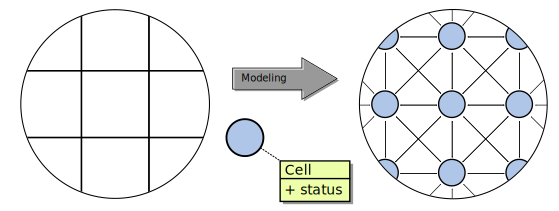
\includegraphics[width=\textwidth]{graphics/30_gol}
  \caption{Cut-out of a Game of Life world (on the left) was modeled as a graph (on
    the right). Each Vertex is described by the vertex property cell, 
    containing the status information of the cell.}
  \label{fig:gol}
\end{figure}



%%%%%%%%%%%%%%%%%%%%%%%%%%%%%%%%%%%%%%%%%%%%%%%%%%%%%%%%%%%%%%%%%%%%%%%%%%%%%%%%
%                                                                              %
% NAMESERVICE                                                                  %
%                                                                              %
%%%%%%%%%%%%%%%%%%%%%%%%%%%%%%%%%%%%%%%%%%%%%%%%%%%%%%%%%%%%%%%%%%%%%%%%%%%%%%%%
\section{Mapping onto the hardware}

%% Requirements
Fact is, that the communication hardware layout is fixed. The access
to the hardware is represented by communicators and these are
connected in the simplest case by an fully connected network, thus
every communicator can send messages to every other
communicator. Therefore a network on top of the communicators has to
be established.

It is a very important property to be able to explicitly map the
communication topologie of the application onto the communication
hardware.

In the first place it should gives the application the possibility to
be optimized on special charakteristics of the compute cluster. For
example could vertices that need to communicate very intensively with
each other can be mapped on neighboring nodes or even onto the same
node. Which makes communication more efficient.

Besides it should be possible to change the mapping of the
communication topologie onto the communication hardware in
runtime. This is important when thinking of occuring unbalanced load
during the run of the application.

%% Process of announce
The objective is to establish a communication overlay on top of the
network provided by the communicators. This overlay network is based
on a graph. Thus all communicators that want to take part on the
communicatin in this overlay need to know this graph.

This Graph can be constructed in parallel by all processes, delivered
by a distributed file system or could even be delivered by some
construction process by explicit communication operations. That is
left open to the user of this library.

The next phase is the distribution of the vertices of the graph to the
processes. This has the meaning that a process responsible for the
communication of this processes. The process will be called host of
the vertices.

The distribution can be done by several methods: randomized, round
robin, dictated by some master process etc. This distribution is again
left open to the user.

Every communicator hosts zero, one or more vertices, so to speak it is
also possible that one communicator host all vertices and communicates
in the end with itself.  Thus the processes announce their hosted
vertices to all other communicators, which will register this
information into their Vertex->Communicators map.  This can be done by
the collective operation allGatherV to the network of communicators.


The NameService is the connection of the graph as the topology
description instance and the communicator as communication hardware
interface.

It contains two mappings. Vertices of a graphs are mapped to
Communicators and Graphs are mapped to contexts.

%% Remapping of vertices
Because the communication hardware and topolgie is seperated,
it is also possible to change the mapping from vertices to 
communicators on runtime. That can be necessary when load
of an application is getting inbalanced during the runtime.

The application can perform a global load balancing step, which
is very similar to static load balancing in the beginning
of the application. Thus vertices are seperated by some rule
and then announced. The difference is, that the communicators
have to send the data of their once hosted vertices to the
new hosts of the vertices.

Another possibility is to do a kind of local load balancing.
This means that communicators hand over vertices to communicators
of adjacent vertices. This might not require a global synchronization
step, instead only local communication with all communicators
that are involved in this local load balancing.

%%%%%%%%%%%%%%%%%%%%%%%%%%%%%%%%%%%%%%%%%%%%%%%%%%%%%%%%%%%%%%%%%%%%%%%%%%%%%%%%
%                                                                              %
% GRAPHCOMMUNICATOR                                                            %
%                                                                              %
%%%%%%%%%%%%%%%%%%%%%%%%%%%%%%%%%%%%%%%%%%%%%%%%%%%%%%%%%%%%%%%%%%%%%%%%%%%%%%%%
\section{Communication on physical domain - GraphCommunicator}
The communication was abstracted from the actual communication layer
and the communicaiton topologie was modeled with a graph and then
maped onto communicators.

The next step is to use the graph as a kind of overlay network and
offer standard communication operations on base of the communicators.

The user should have the feeling, that he really is exchaning messages
between the vertices of the graph and the library is taking care, that
the messages are reaching the correct vertex. Thus this is the level
of abstraction with which the user interacts.

% Communication schemas
Communication on base of a graph is an interaction of the NameService
and the graph on which should be communicated. The Graph represents
connected communication partners and therefore also determines which
vertices are able to communicate with each other. The NameService
delivers the information on which Communicator the vertices are
located.

Vertices are peers of the communication network and can be addressed
directly.

Thus the interface for direct communication involves the graph in
which context is communicated, the vertex which is receiver or sender
of data and the transmited data itself. An overlay based on Graphs
with multiedge support also needed to add the according edge between
two communicating vertices.

Operations between all vertices of a graph can be performed as
collective operations on the graph.  In the case some collective
operation should be performed, a communicator is responsible to start
the collective operation for its hosted vertices otherwise it blocks
all other communicators.

Collective operations add some more arguments to the communication
interface.

\begin{itemize}
\item Gather - Vertices on the same host collect data local first and
  then use the collective gather provided by the communicator
\item Reduce - Vertices on the same host reduce data local first and
  then use reduce provided by the communicator.
\item Synchronize - This is a barrier function which lets the host
  wait for all others host that are contributing to a special graph.
\item There is some problem with these collective operations when a
  host forgets to call the collective on all its hosted vertices of an
  graph.  Then the collective operation can not be finished and the
  application is therefore locked. This problem is passed wo wise
  programmers which do not forget this issue.
\end{itemize}



%%%%%%%%%%%%%%%%%%%%%%%%%%%%%%%%%%%%%%%%%%%%%%%%%%%%%%%%%%%%%%%%%%%%%%%%%%%%%%%%
%                                                                              %
% ETC                                                                          %
%                                                                              %
%%%%%%%%%%%%%%%%%%%%%%%%%%%%%%%%%%%%%%%%%%%%%%%%%%%%%%%%%%%%%%%%%%%%%%%%%%%%%%%%

\subsection{Requirements for the upcoming generation of super computers}
\begin{itemize}
\item Run picongpu on xeon phi in native mode
\item Exchangeable communication layer to be portable / ready for the
  upcoming generation of acceleration devices
\end{itemize}


The during this thesis developed communication layer was leaded by the
needs of PIConGPU as an example application for high performance
computing on cluster systems.

The implementation of PIConGPU has some lack of abstraction for their
communication. Because there is no abstraction layer which hides the
MPI communication calls, which makes it impossible to exchange it.

Also the communication topology of the simulations is not be modeled
satisfying. Neighboring subdomains are directly addressed by their
ranks, thus changing the communication topology also leads to a lot of
changes in the algorithm.



\cleardoublepage

%%% Local Variables:
%%% TeX-master: "diplom"
%%% End:
